\section{Concept of Root Loci}

\begin{frame}
\frametitle{Concept of the method}
In this chapter the Root Locus Method is presented. This technique shows how changes in the system's feedback characteristics and other parameters influence the pole locations. The method permits us to plot the locus of a closed-loop pole location in the s-plane as a parameter varies, which will produce a root locus (hence the name of the technique).\\
\vspace{1em}
It is very important to understand the background of root loci: how they take their shape, why they are useful, ... Therefor, we start this chapter by explaining the concept of the Root Loci Technique. Next we explain how to sketch a root locus. Finally we will give some examples in MATLAB.
\end{frame}

\begin{frame}
\frametitle{Concept of the technique}
	We begin with the basic feedback system, shown in the figure below:
	\begin{figure}
		\centering
		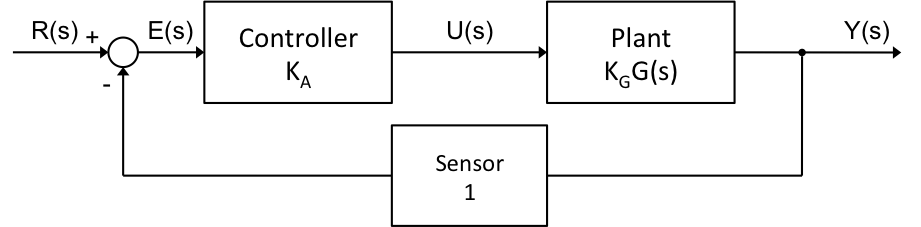
\includegraphics[width=1\linewidth]{closed_loop_diagram}
	\end{figure}
	The closed-loop transfer function is:
	\begin{center}
		$H(s) = \frac{Y(s)}{R(s)} = \frac{K_AK_GG(s)}{1 + K_AK_GG(s)}$.
	\end{center}
\end{frame}

\begin{frame}
\frametitle{Concept of the technique}
	Looking at this transfer function, we can conclude that the closed-loop roots depend on the amplifier gain $K_A$. We can now plot the locus of all possible roots of the characteristic equation: 
	\begin{center}
		$1 + K_AK_GG(s) = 0 \hspace{1em} (10.1)$
	\end{center}
	as $K_A$ varies form $0$ to $\infty$. This results in a graph which can help us in selecting the best value of $K_A$.\\
	\vspace{1em}
	Furthermore, by studying the effects of additional poles and zeros, we can determine the consequences of additional dynamics in the loop. We can also extend this technique to examine the effect of other plant-parameter changes in order to achieve the best overall control design.
\end{frame}

\begin{frame}
\frametitle{Root Locus}
	\begin{block}{Definition 1}
		The root locus is the set of values of s for which $1 + KG(s) = 0$ is statisfied as the real parameter $K$ varies from $0$ to $+\infty$. Often $G(s)$ is the open-loop transfer function of a system; in this case, roots on the locus are closed-loop poles of that system.
	\end{block}
	\begin{block}{Definition 2}
		The root locus of $G(s)$ is the set of points in the s-plane where the phase of $G(s)$ is $180$degrees.	
	\end{block}
	\begin{block}{Use of root loci}
		The root loci method provides a tool not only for selecting the gain but for designing the dynamic compensations as well.
	\end{block}
\end{frame}

\begin{frame}
\frametitle{Concept of the technique}
	For the further derivation, we assume that the system's open-loop transfer function $K_GG(s)$ is a rational function whose numerator is $K_Gb(s)$ and whose denominator is $a(s)$.$b(s)$ is a monic polynomial of degree $m$ and $a(s)$ is a monic polynomial of degree $n$ such that $n \geq m$.\\
	\vspace{1em}
	We assume the plant gain $K_G$ to be positive and define the root-locus parameter K as:
	\begin{center}
		$K = K_AK_G$
	\end{center}
\end{frame}

\begin{frame}
\frametitle{Concept of the technique}
\begin{block}{Root-Locus form}
	We can express equation (10.1) in different equivalent ways:
	\vspace{-1em}
	\begin{align*}
		1 + KG(s) &= 0,\\
		1 + K\frac{b(s)}{a(s)} &= 0,\\
		a(s) + Kb(s) &=0,\\
		G(s) & = -\frac{1}{K}.
	\end{align*}
\end{block}

\begin{alertblock}{Open-loop vs Closed-loop}
	The root-locus method can be thought of as a method for inferring properties of the closed-loop system given the open-loop transfer function $KG(s)$.
\end{alertblock}
\end{frame}

\begin{frame}
	\begin{example}
		\textbf{Problem}: a normalized transfer function of a DC motor is:
		\begin{equation}
		K_GG(s) = \frac{1}{s(s+1)}.
 		\end{equation}
 		Solve for the locus of roots with respect to $K_A$ of the closed-loop system created by feeding back the output as shown in the figure:
 		\begin{figure}
 			\centering
 			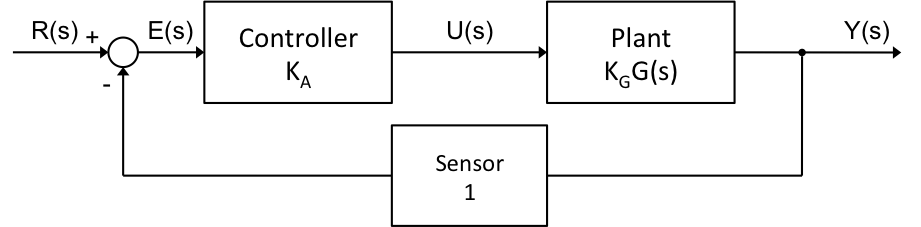
\includegraphics[width=0.8\linewidth]{closed_loop_diagram}
 		\end{figure}
 		Solve by using direct calculations of the root locations.
	\end{example}
\end{frame}

\begin{frame}
	\begin{exampleblock}{}
		\textbf{Solution}: in terms of our notation
		\vspace{-0.5em}
		\begin{columns}
			\begin{column}{0.2\textwidth}
				\begin{align*}
				m &=0,\\
				n &=2,
				\end{align*}
			\end{column}
			\begin{column}{0.2\textwidth}
				\begin{align*}
				K_G =1,\\
				K_A =K,
				\end{align*}
			\end{column}
			\begin{column}{0.2\textwidth}
				\begin{align*}
				b(s) =1,\\
				a(s) = 1.
				\end{align*}
			\end{column}
		\end{columns}
		\vspace{1em}
		We can use the root-locus form $a(s) + Kb(s) = 0$ to obtain a quadratic equation of which the roots will produce a graph.\\ 
		In this case, the quadratic equation:
		\begin{equation}
		s^2 + s + K = 0
		\end{equation}
		has roots:
		\begin{equation}
		r_1,r_2 = -\frac{1}{2} \pm \frac{\sqrt{1 - 4K}}{2}.
		\end{equation}
	\end{exampleblock}
\end{frame}

\begin{frame}
	\begin{exampleblock}{}
		The root locus is shown below
		\begin{figure}
			\centering
			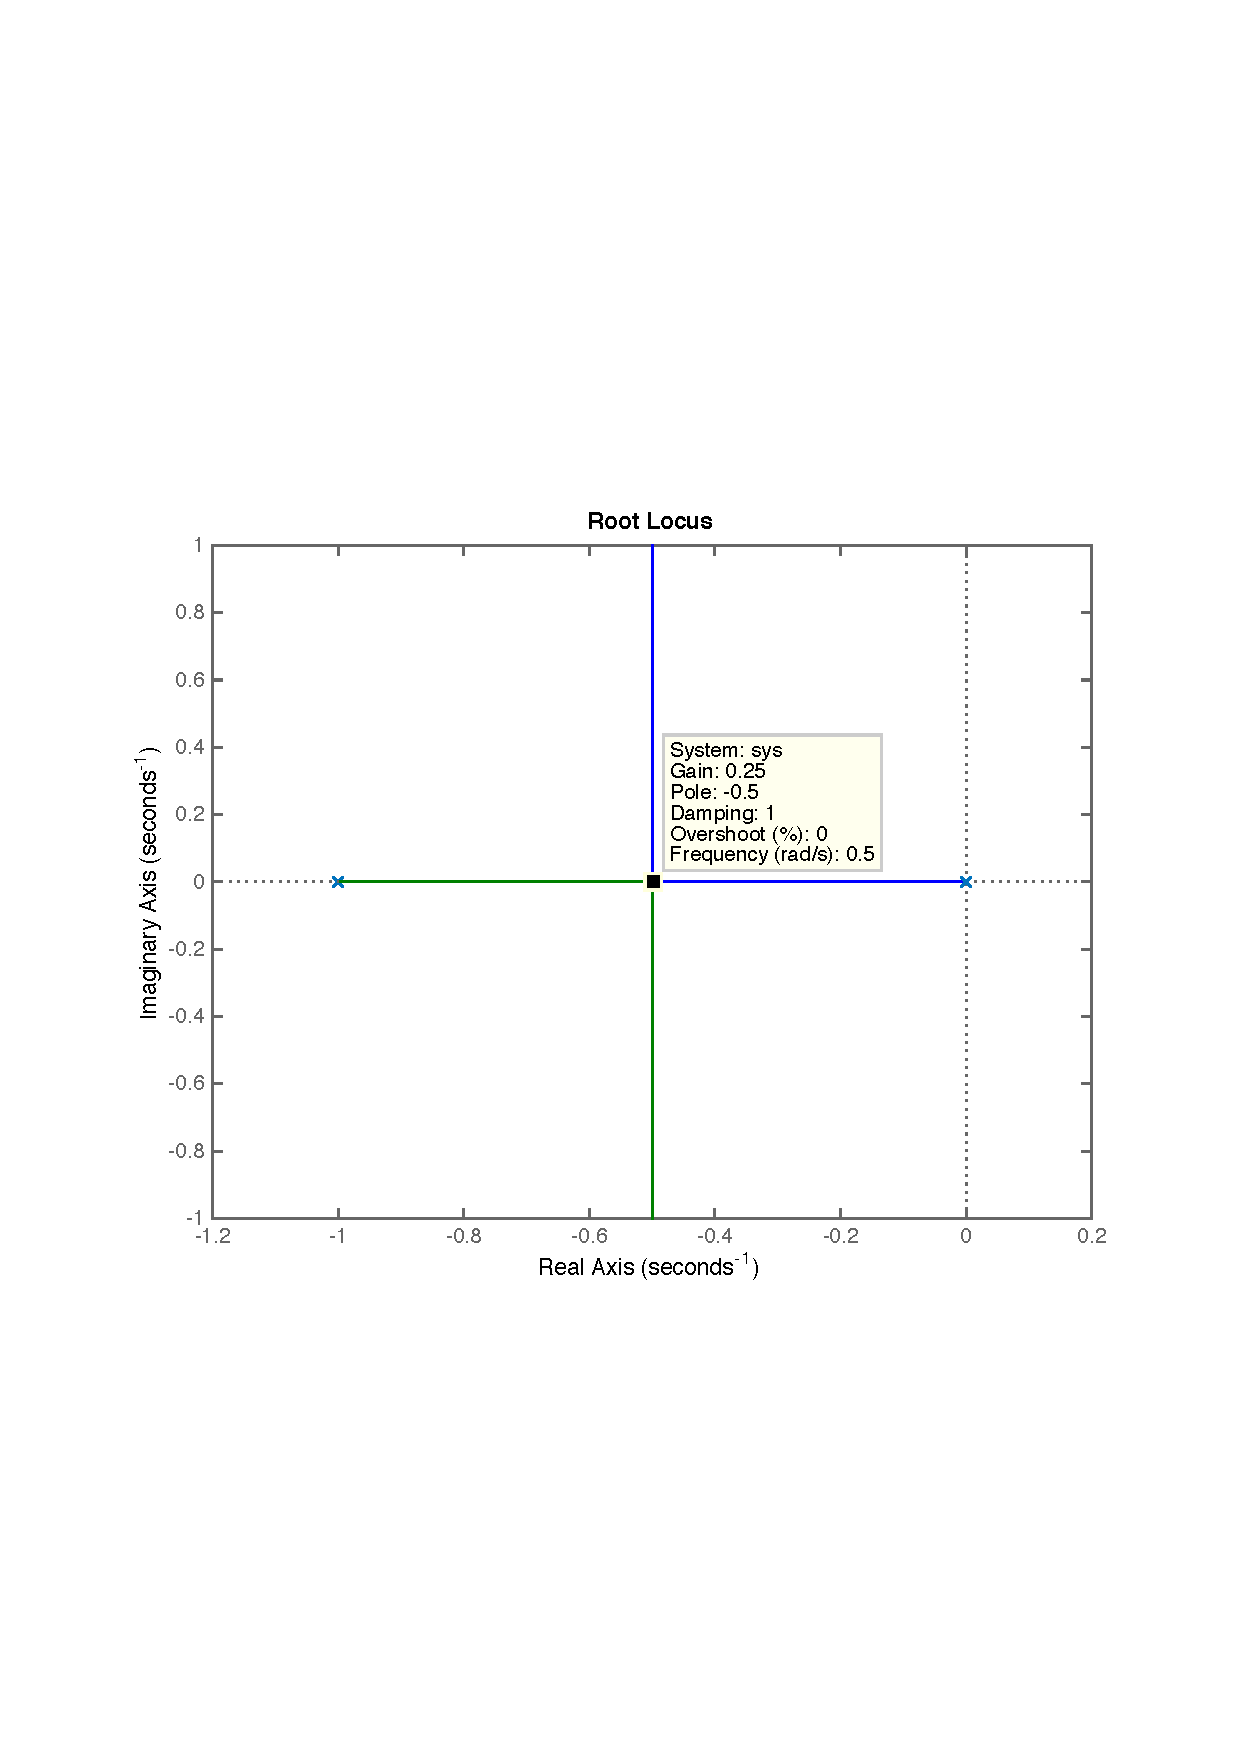
\includegraphics[width=0.7\linewidth]{root_locus_ex1}
		\end{figure}
	\end{exampleblock}
\end{frame}

\begin{frame}
	\begin{exampleblock}{}
		\begin{itemize}
		\item For $0\leq K \leq \frac{1}{4}$, the roots are real between $-1$ and $0$;
		\item At $K = \frac{1}{4}$ there are two roots at $-\frac{1}{2}$;
		\item For $K>\frac{1}{4}$ the roots become complex, with a real part of $-\frac{1}{2}$ and an imaginary part that increases essentially in proportion to the square root of K
		\end{itemize}
		\vspace{1em}
		We can now compute K at the point where the locus crosses $\zeta = 0.5$: we know that if $\zeta = 0.5$, then $\theta = 30$degrees and the magnitude of the imaginary part of the root is $\sqrt{3}$ times the magnitude of the real part. The magnitude of the real part is $\frac{1}{2}$ and thus, we have: \begin{equation}
		\frac{\sqrt{4K - 1}}{2} = \frac{\sqrt{3}}{2}
		\end{equation}
		and therefor, $K = 1$.
		\end{exampleblock}
\end{frame}

\section{How To Draw Root Loci}

\begin{frame}
	INCLUDE SLIDES WITH EXPLANATION FOR EACH STEP
\end{frame}

\begin{frame}
	\frametitle{Overview of the guidelines}
	\begin{enumerate}
		\item Mark poles with $\times$ and zeros with $\circ$;
		\item Draw the locus on the real axis to the left of an odd number of real poles plus zeros;
		\item Draw the asymptotes, centered at $\alpha$ and leaving at angles $\phi_l$, where:
		\begin{itemize}
			\item $n - m$ = number of asymptotes\\
			\item $\alpha = \frac{\varSigma p_i - \varSigma z_i}{n-m}$\\
			\item $\phi_l = \frac{180° + 360°(l - 1)}{n - m}, l = 1,2,...,n-m.$
		\end{itemize}
		\item CONTINUE WITH STEP 4
	\end{enumerate}
\end{frame}

\section{Root Loci and MATLAB}

\begin{frame}
	INCLUDE SLIDES WITH MATLAB EXAMPLES
\end{frame}